\subsection{Simulation of AFM Imaging\label{Chapter 2: ABAQUS Simulation of AFM Raster Scan}}

\subsubsection{General Scan Dynamics for Imaging}

Following the application of FEM to single indentations, similar simulations were created to extend to AFM imaging. Independent ABAQUS simulations were produced in which individual indentations at positions across the surface's domain replicate the dynamics of an AFM raster-scan. Our AFM simulation subdivides the XY domain of the geometry into bins to produce the scan positions. The initial vertical heights of the indenter are then calculated at each position. Next, the independent ABAQUS simulations for the indentation at each position are produced, and corresponding vertical forces and displacements are extracted. This provided a four-dimensional array of indenter positions and corresponding force over the surface. Subsequently, computation of the contours for a given reference force produces the final AFM images shown in Figure \ref{fig: TestRasterScan}. This methodology is computationally efficient as it utilises the initial heights computed from hard-sphere contact, resulting in the indentation data being consistently calculated to the same depth across the entire surface. This is as the hard-sphere contact represents the tangent points of the two surfaces' across the scan.

\begin{figure}[H]
\centering

    \begin{subfigure}{0.49\textwidth}
        \centering
        \caption{ \label{fig: TestRasterScan-Positons} }   
        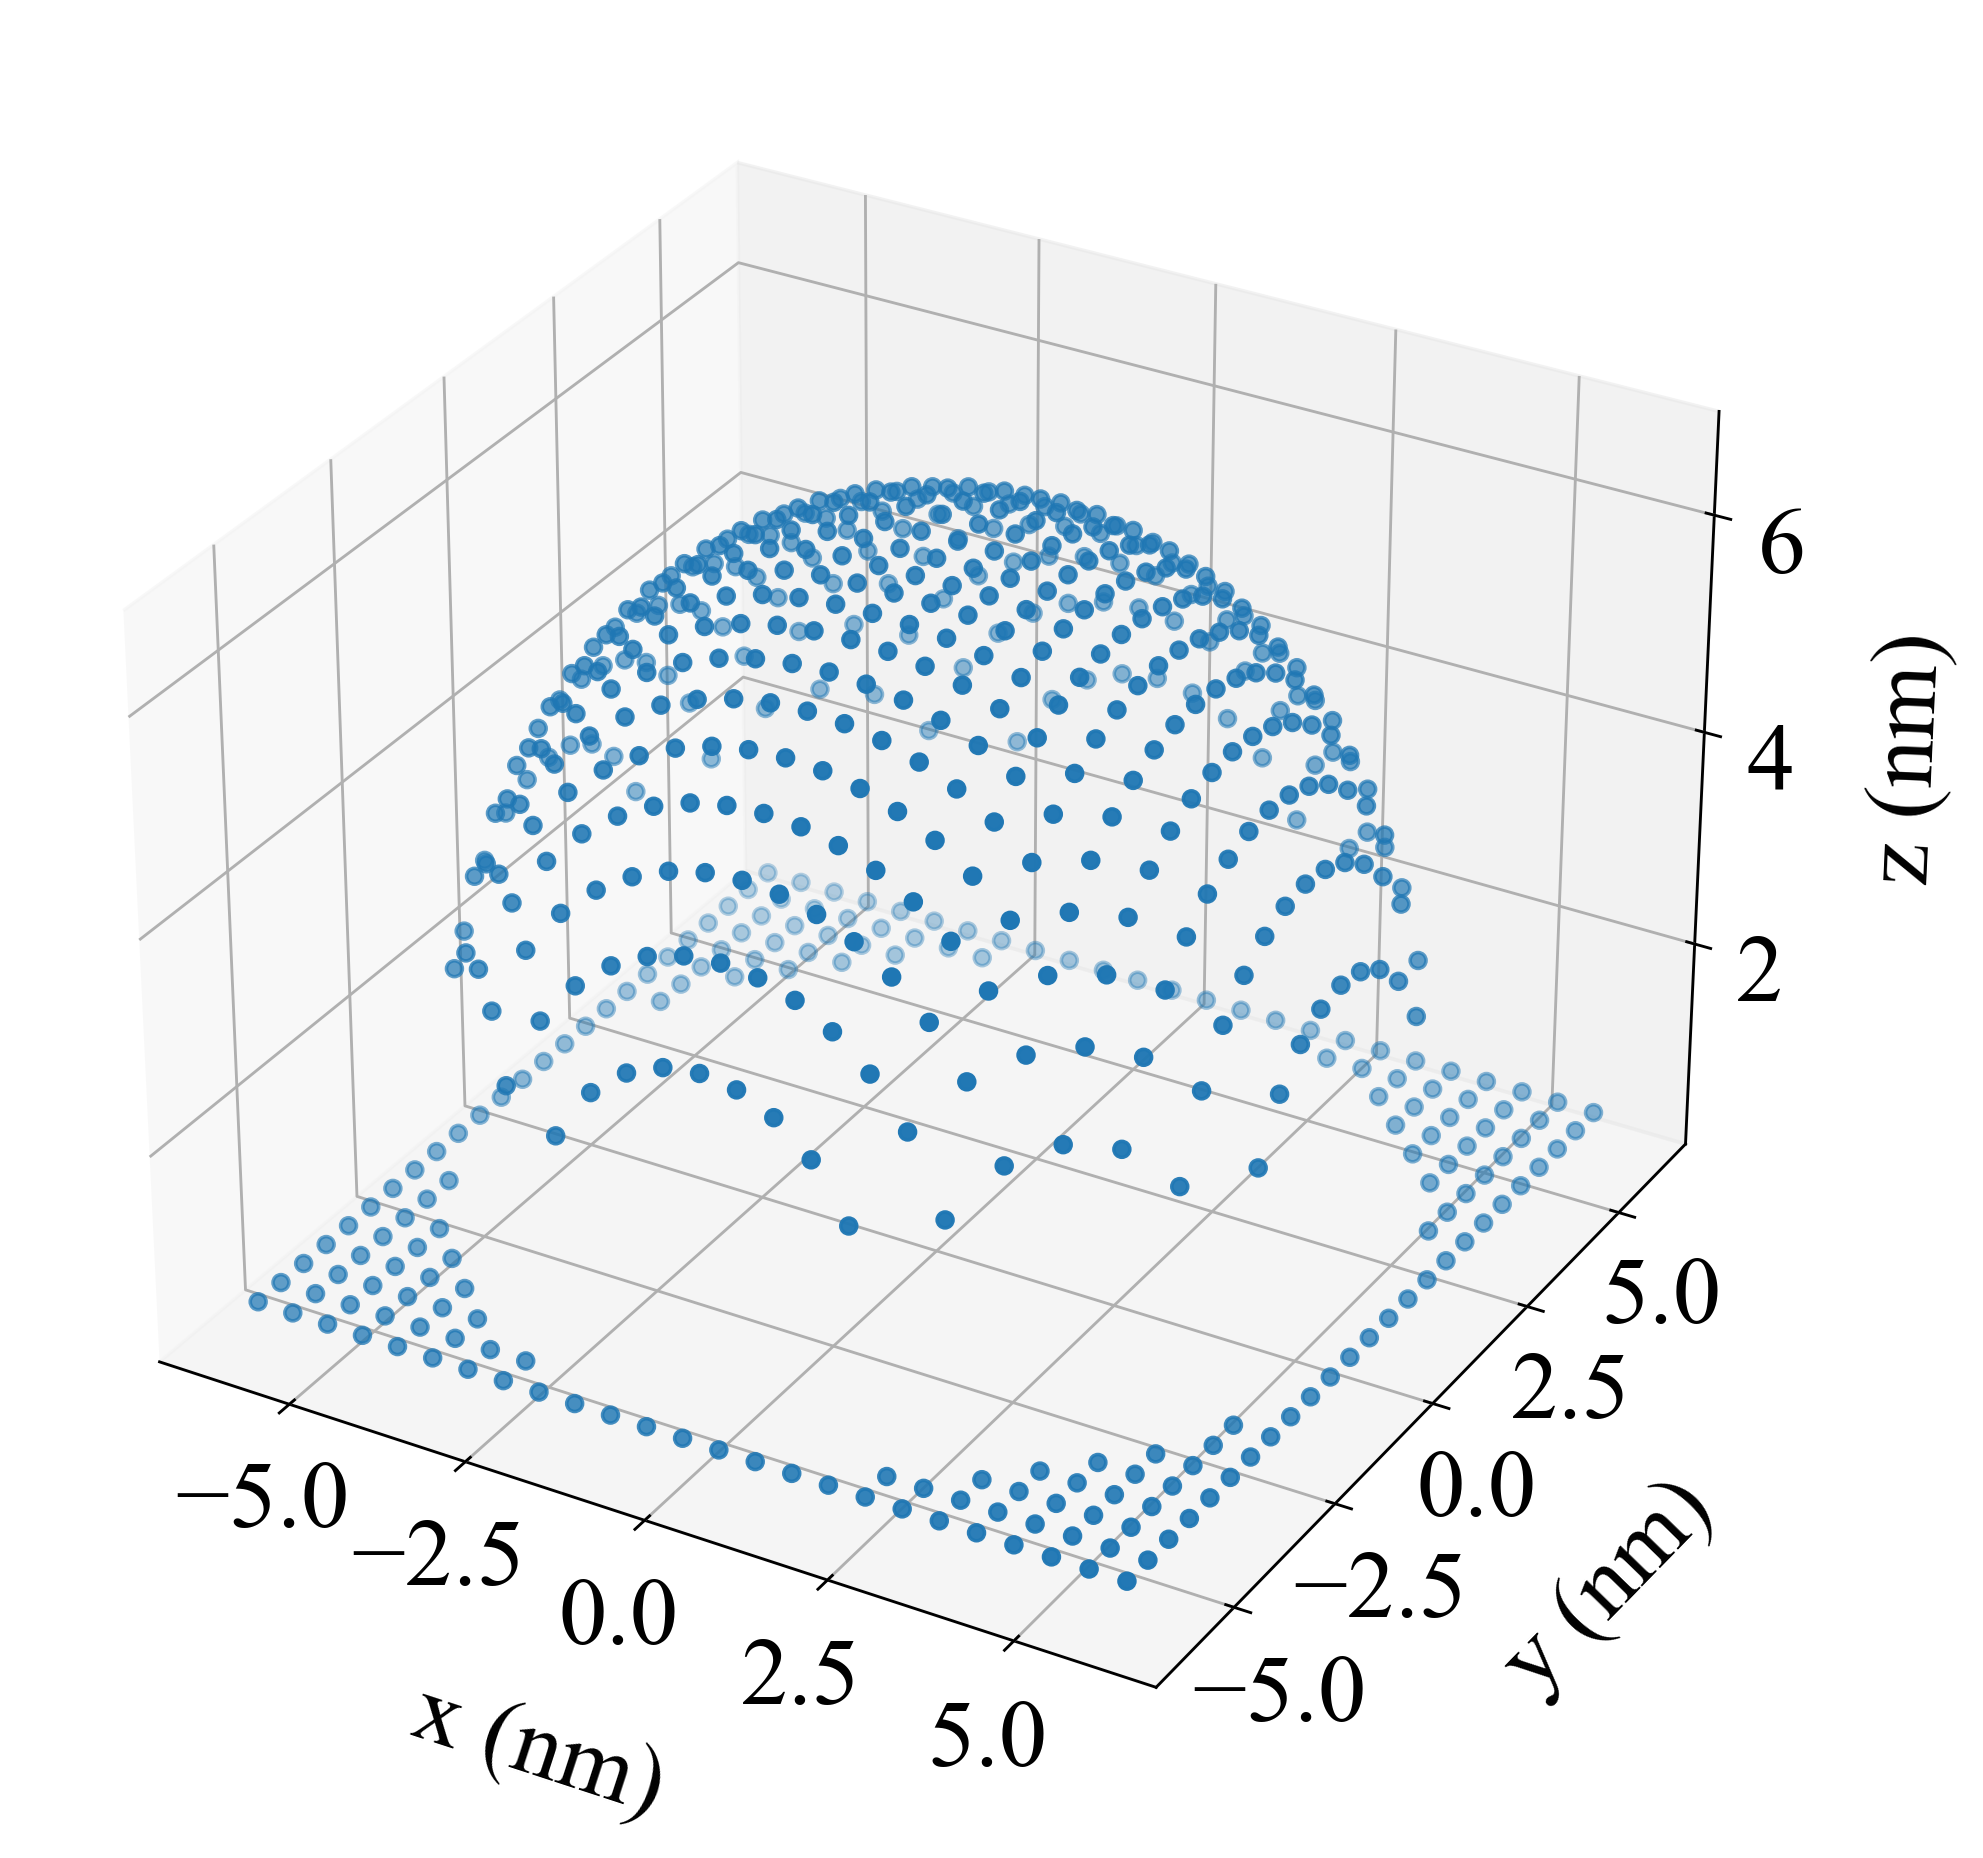
\includegraphics[width=1\linewidth]{Figures/TestRasterScan-Positons.png}
    \end{subfigure}
    \hfill
    \begin{subfigure}{0.49\textwidth}
        \centering
        \caption{\label{fig: TestRasterScan-Results}  }
        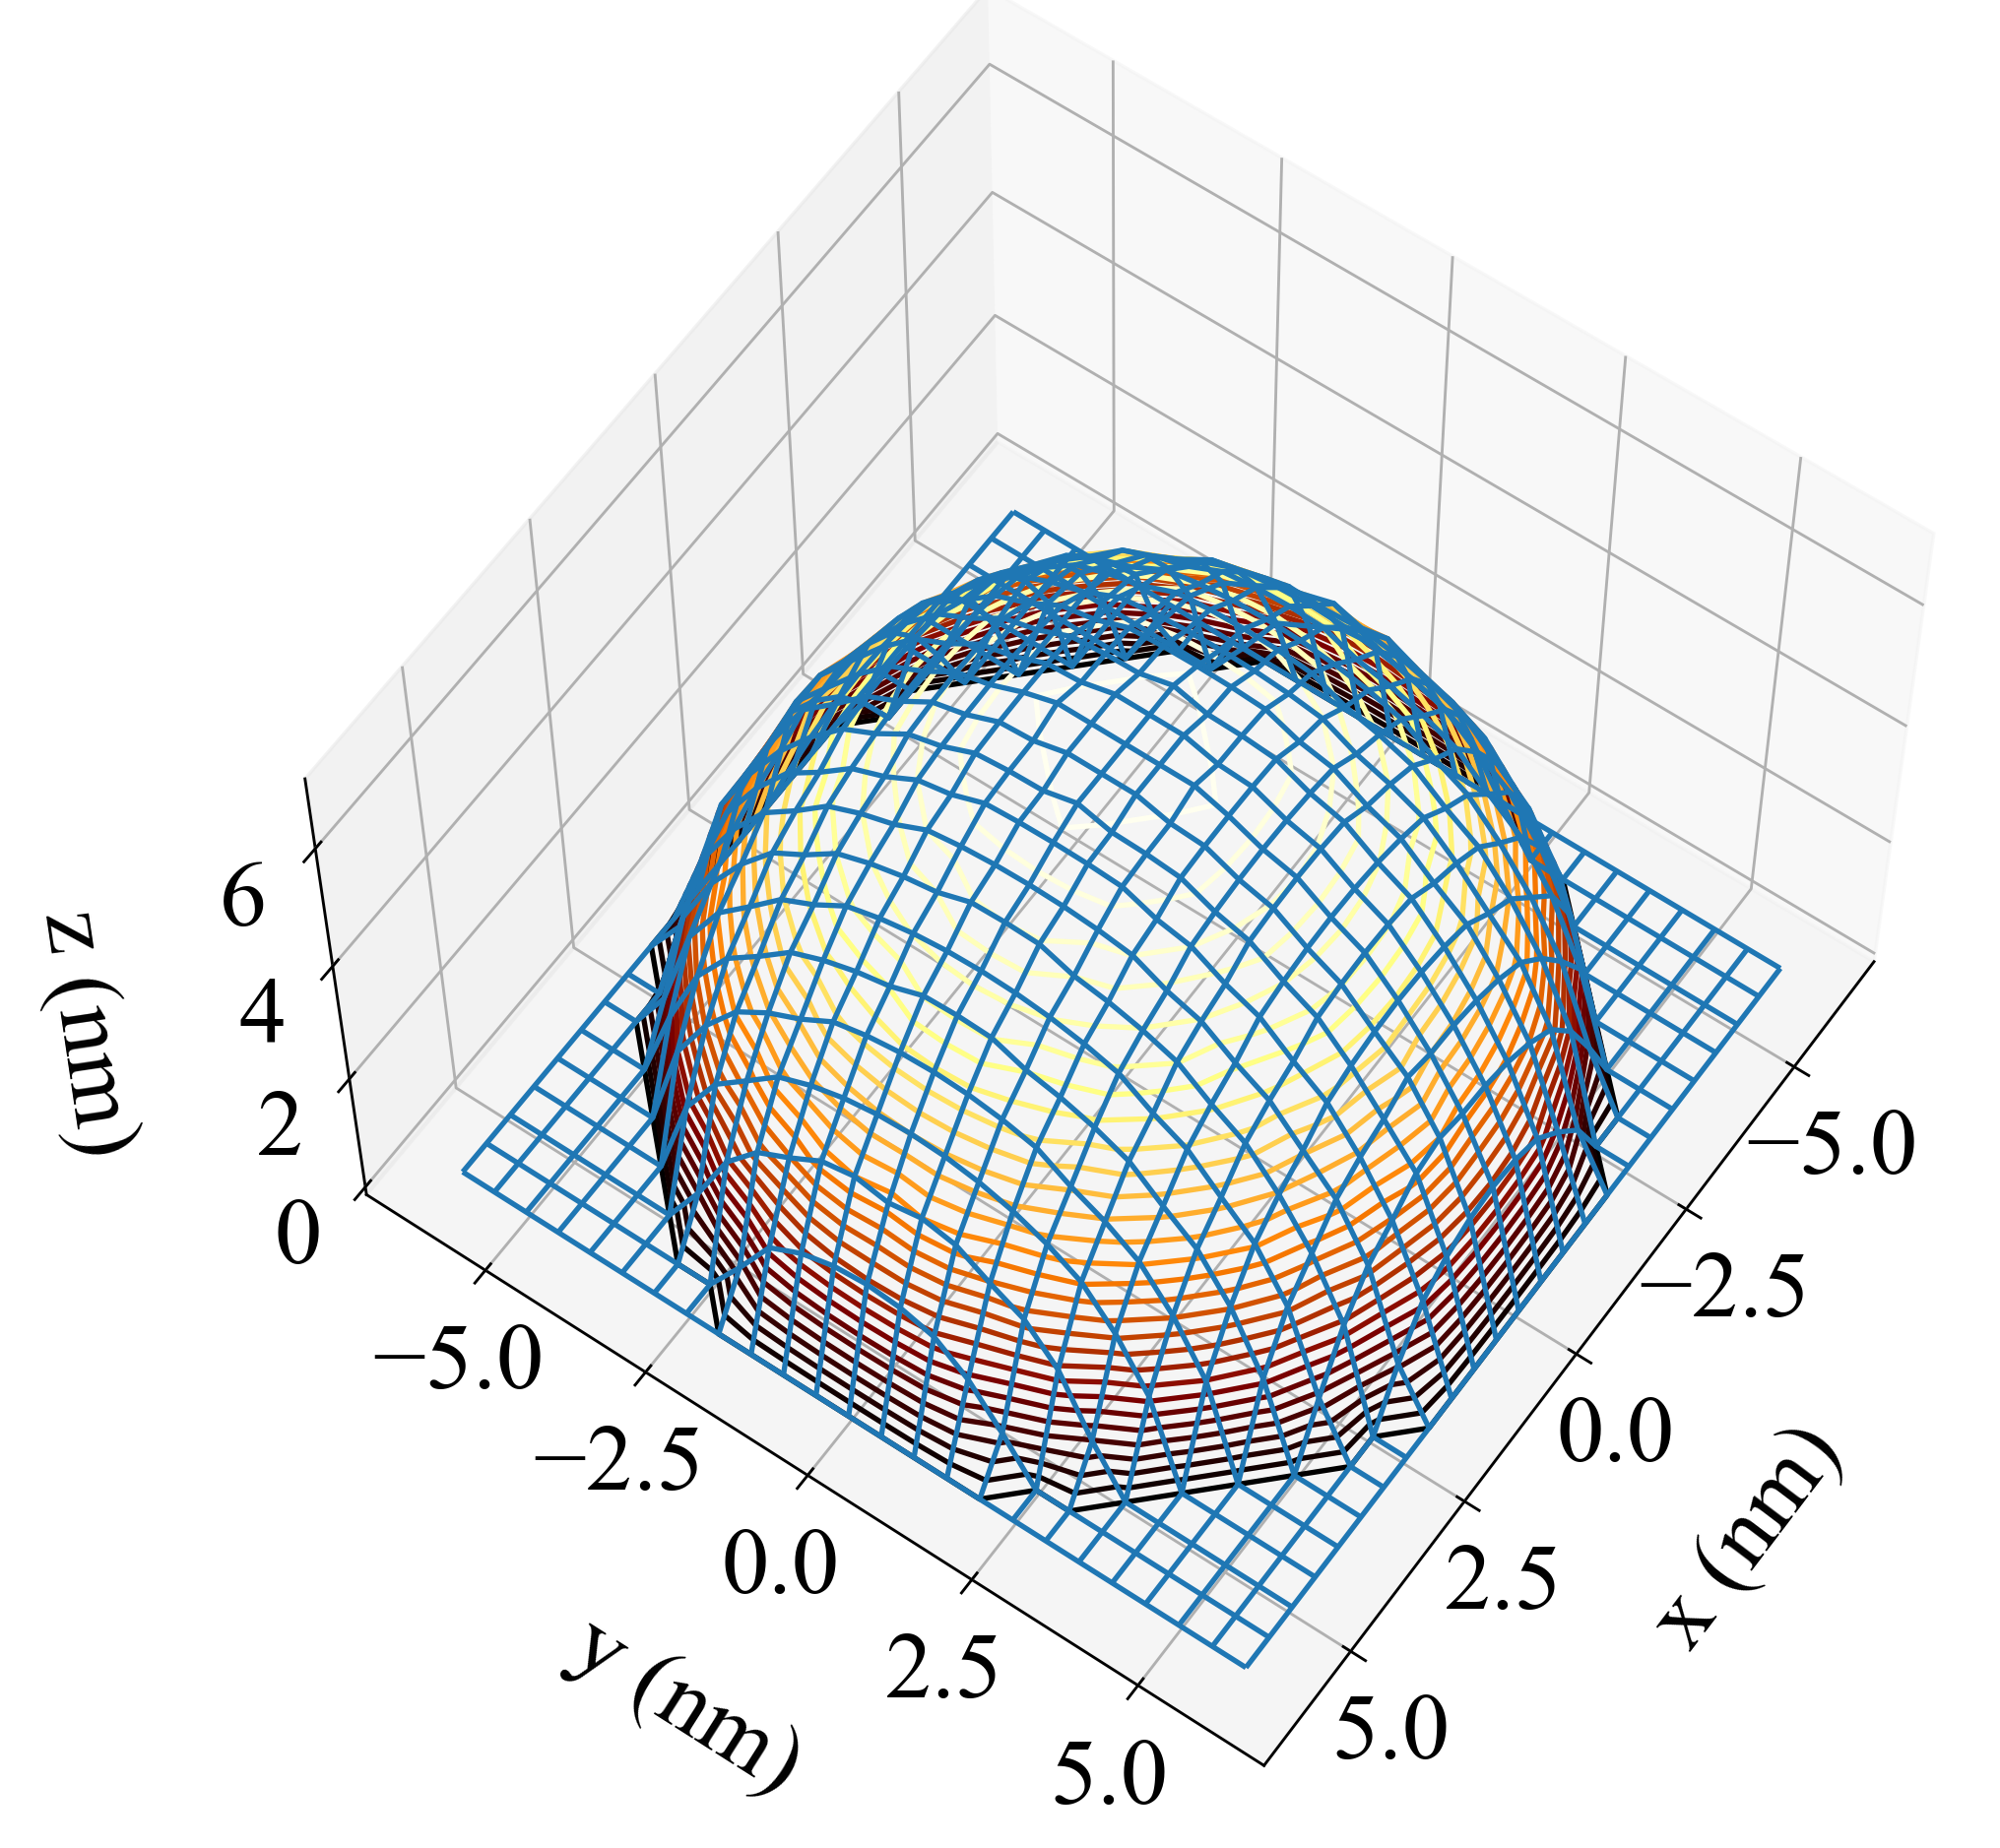
\includegraphics[width=1\linewidth]{Figures/TestRasterScan-Results.png}
    \end{subfigure}
    \hfill
    \begin{subfigure}{0.89\textwidth}
        \centering
        \caption{\label{fig: TestRasterScan-AFM}  }
        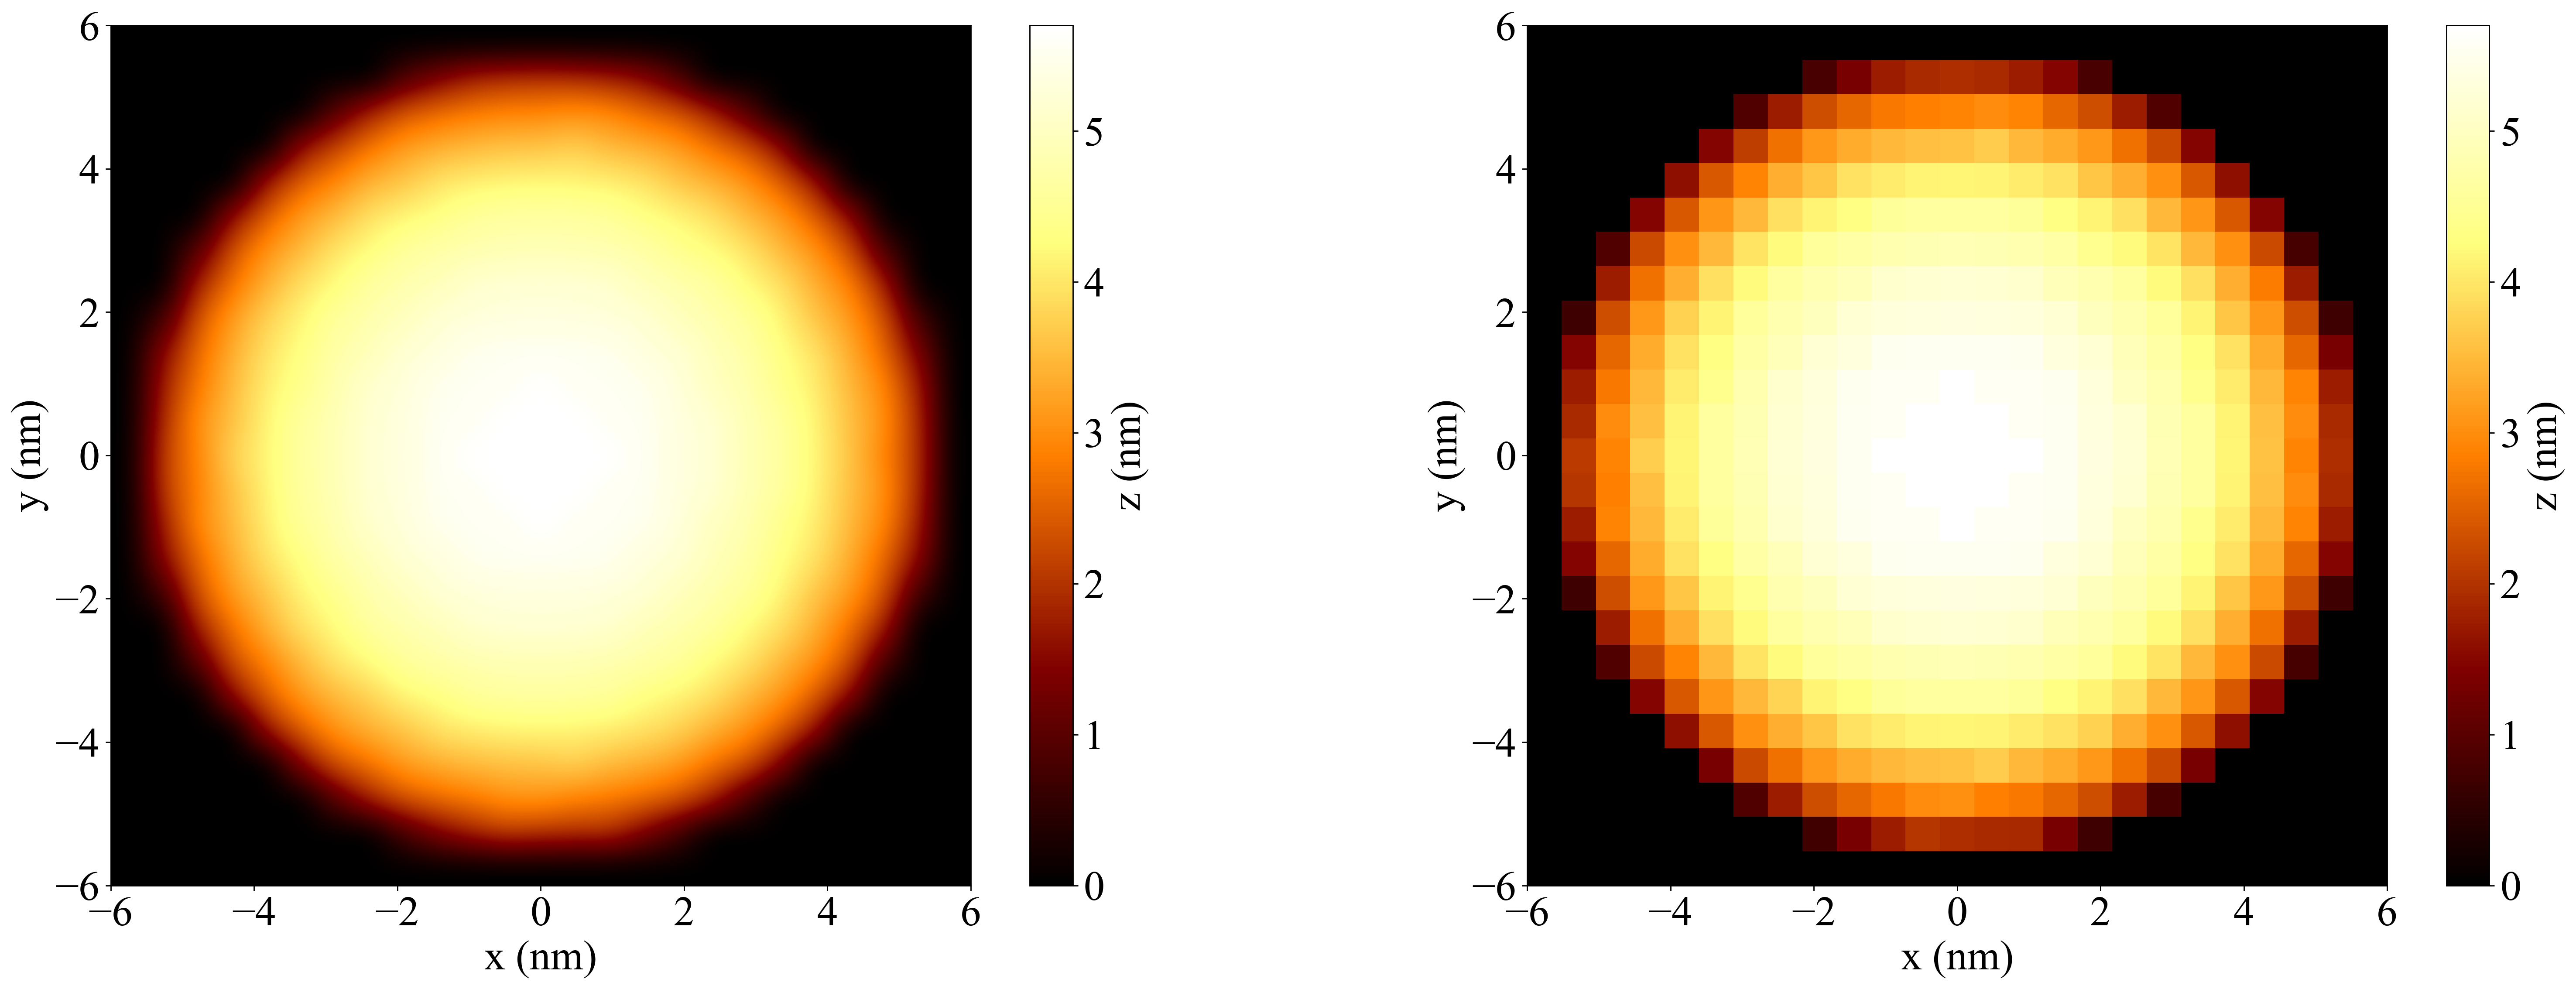
\includegraphics[width=1\linewidth]{Figures/TestRasterScan-AFM.png}
    \end{subfigure}

    
    \caption{\label{fig: TestRasterScan}Plots for simulated AFM image on a hemisphere of radius r=5nm. $E=1000KPa$, $\nu =0.3$, and scan bins of 0.5nm. (A) Vertical initial scan positions for hemisphere. (B) Three-dimensional plot of force contours for 100pN for simulated AFM image. (C) Simulated 2D heatmap AFM image for 100pN force. Left: Interpolation. Right: Raw data }
\end{figure}

\subsubsection{Image Processing and Interpolation}

The pseudo-AFM images are produced from two-dimensional arrays of surface heights over the XY grid of scan positions. These heights map the surface contour of equal force over the scan. These contours are calculated from the indentation depth and force arrays produced by the ABAQUS/FEM simulations. For a given threshold/ reference force, the corresponding depths are found using a list comprehension (see Figure \ref{fig: FourceContours}). The list comprehension iterates over the force data for each scan position and compares it with the reference force. The index for the value equal or greater than the reference force is found and the corresponding depth is stored. This is used to calculate the surface heights. If no values in the force array for a scan position are greater than the reference force, the function sets the corresponding contour value to the maximum indented depth. The contour data is then reshaped into the 2D grid representing the scan positions. Subsequently, the Matplotlib imshow function is used to produce the visualisation with a Colormap to illustrate the variation in surface heights. Normalisation of the colourmaps applies either linear scaling over the domain or power normalisation depending on detail contrast. Moreover, to increase pixel density images are interpolated using Mathplotlib imshow functions in-built bicubic interpolation.

\begin{figure}[H]
\centering
    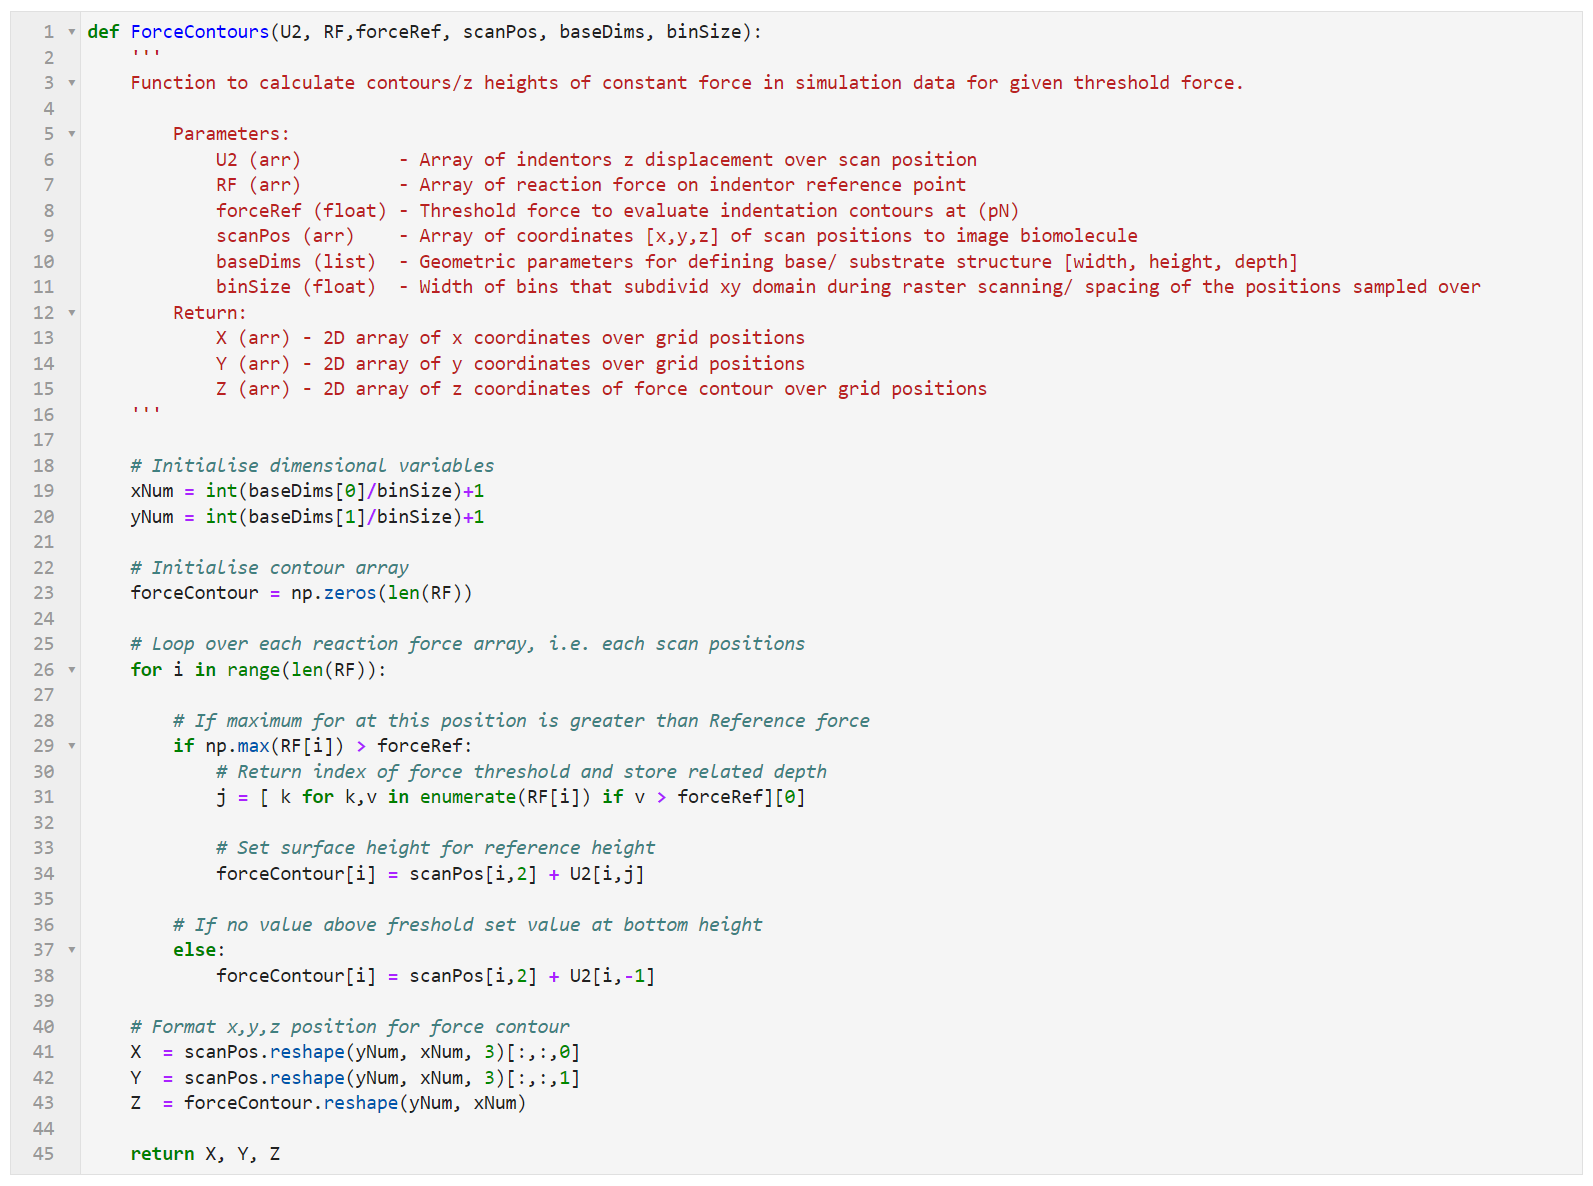
\includegraphics[width=1\linewidth]{Figures/ForceContours.png}
    \caption{\label{fig: FourceContours}Code Snippet showing the calculation of force contours for AFM image. For a given threshold/ reference force, the corresponding depths are used to calculate the surface heights over the scan positions.}
\end{figure}


\subsubsection{Application to Biomolecules \label{Chapter 2: ABAQUS Simulation of AFM Biomolecules}}

The application of these dynamics to biomolecules requires some simple modifications. Biological structures are produced using Protein Data Bank (PDB) files that specify the constituent atoms of a biomolecule and the corresponding coordinates. As the simplest approach, the biomolecule is modelled as an elastic material produced from the assembly of spheres (with van der Waals radius) of the individual atoms. The structure is assumed to be a continuous, homogeneous and isotropy material, with a typical biological Young's Modulus and Poisson ratio of 1000KPa and 0.3, respectively. The molecule is partially embedded in a rigid base/ substrate, and the scan positions are then calculated over the domain of the base. The embedded portion simulates a soft molecule absorbed onto a solid support and the molecule is then fixed at its base using boundary conditions. The AFM probe tip is modelled as a rigid capped conical indenter where the indentation is non-slip and without adhesion. The contact is modelled as "surface to surface" type, with the properties of hard contact in the normal direction and "frictionless" in the tangential direction to ensure no slip and no adhesion. Indentation data from the indenter is mapped and sampled via reference points at the centre. The computations were quasi-static with an implicit algorithm and using R3D10 tetrahedral elements (generally greater than 100,000). The elastic constitutive relations are integrated with the main body of the Abaqus code. 

The initial scan positions must be calculated numerically as PDBs only provide atom positions, not surface structure. The XY scan positions are produced by creating a rectangular grid of positions over the base, each separated by a predefined bin size. The heights at each position are calculated by setting the tip above the sample and calculating the minimum vertical distance between the tip and the molecule's surface (corresponding to the tangent point of the two surface's). Figure \ref{fig: ScanPositions} illustrates the calculations made by the code. For each scan position, a loop is used to calculate the radial distances to the atoms in the biomolecule (shown as $R_{Interact}$ in Figure \ref{fig: ScanPositions}). If the atom lies within the indenters boundary ($R_{Boundary}$), the atom and indenter could interact. Therefore, the vertical distances between the surface of the indenter and the "interacting atoms" of the molecule are computed. This produces an array of "dz" values which represents all differences in height between the tip and portion of molecule located within the boundary of the indenter. As illustrated in Figure \ref{fig: ScanPositions}, the minimum of these values gives the vertical distance corresponding to the position where the tip is in tangential contact. Subsequently, using this minimum dz value the tangent points for a scan location can be calculated. Repeating this for all scan locations provides an array of coordinates [x,y,z] of scan positions. For computational efficiency, this can be clipped to only include positions where the tip and molecule interact.

\begin{figure}[H]
\centering
    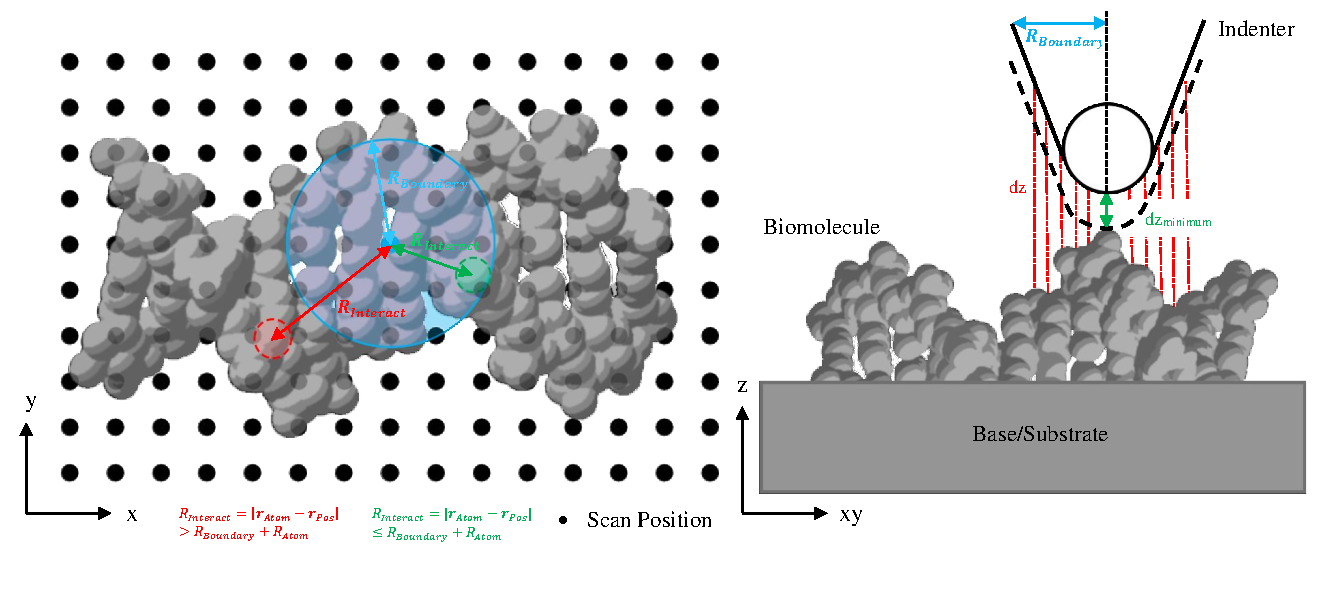
\includegraphics[width=1\linewidth]{Figures/ScanPositions diagram.pdf}
    \caption{\label{fig: ScanPositions}Schematic diagrams illustrating the calculation of initial scan heights in AFM code. Left: Illustrates the calculation atoms on the surface within the indenters boundary. Black dots represent the XY grid of scan positions. The calculation is restricted to the XY plane in which only atoms inside the radial extent of the indenters, $R_{Boundary}$ (blue), are calculated. The red atom represents an atom outside the extent and thus is omitted, as appose to the green atom, which is included. Right: Illustrates calculation of heights for each given position. An array of all distances (dz) between the indenters and molecules surfaces are calculated (red). The minima of these distances thus give the translation distance to place the indenter in tangential contact.}
\end{figure}

An outline of the simulation script is shown in Figure \ref{fig: Code Flowchart}. The code has three main phases: In the preprocessing phase, the desired PDB file is imported via the PDB function and used to process the biomolecule's structure in the MolecularStructure function. Subsequently, the base and indenter geometry is calculated, and the ScanGeometry function determines scan positions for the simulation. These variables and other predefined simulation variables are exported to CSV files using the ExportVariables function. Finally, the CSV files and the ABAQUS scripts are transferred to the remote server where the simulations are carried out. There are 3 ABAQUS scripts run in the submission phase. First, the SurfaceModel and RasterScan scripts are run sequentially using the RemoteCommand function. These scripts produce the ABAQUS surface model and input files for simulations at each scan position. Next, the BatchSubmission function creates a script to run the input files sequentially on the remote server. Once the simulations are complete, the data is stored in ODB files. Running the ODBAnalyis script extracts the indentation data and exports it to CSV files. Once completed, the simulation data can be transferred back to the local machine, where it is processed. In the postprocessing phase, the Data Processing function extracts data from the CSV files and formats the data to include all scan positions. The ForceContour function subsequently calculates the surface heights for a given reference force. Finally, this is plotted in an AFM image using ContourPlot function. (See Appendix \ref{Appendix: ABAQUS Script} for complete code).

\begin{figure}[H]
\centering
    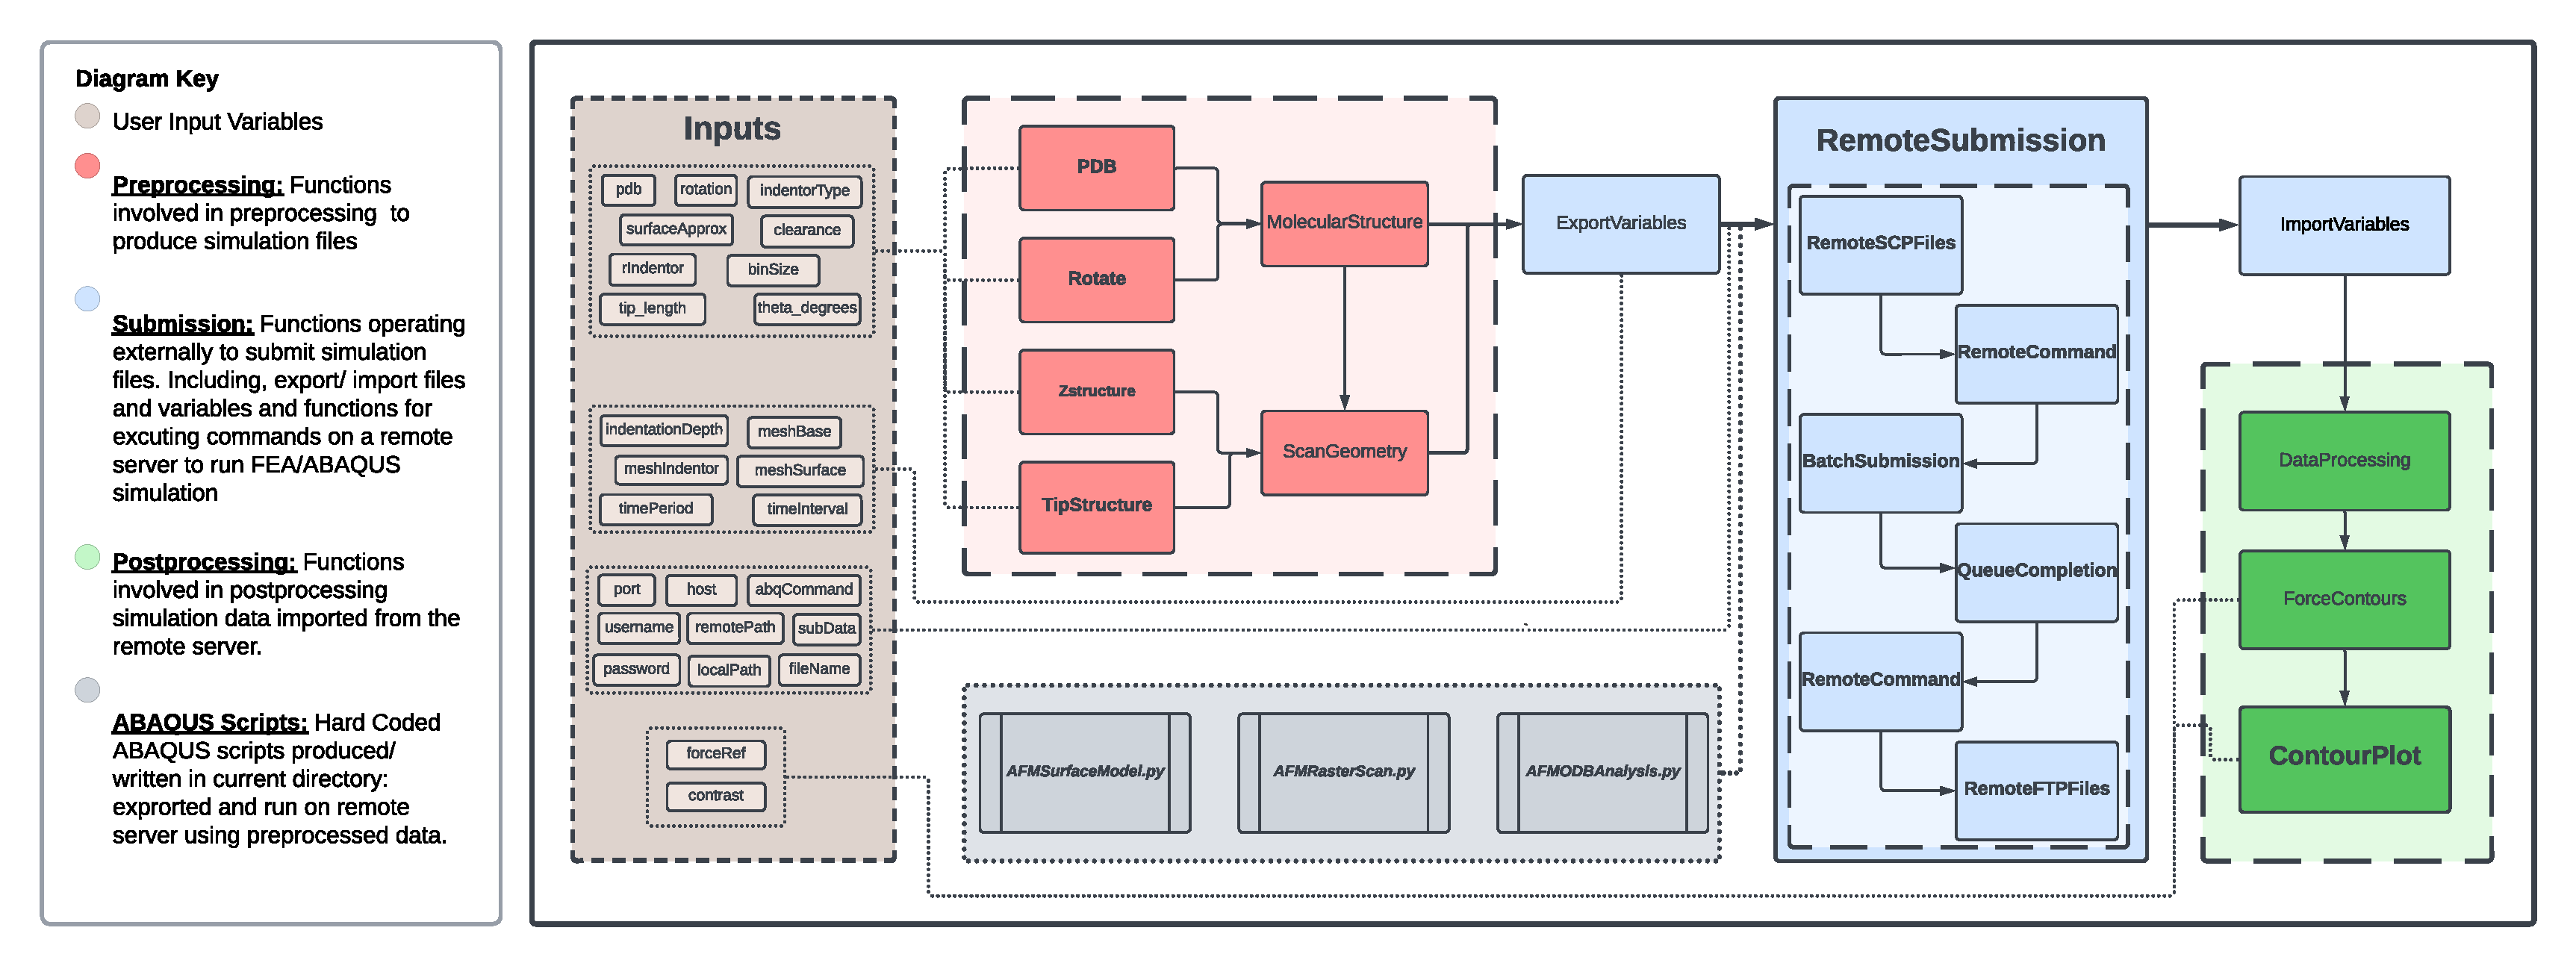
\includegraphics[width=1\linewidth]{Figures/AFM Simulation Code Flow chart.pdf}
    \caption{\label{fig: Code Flowchart}Flow diagram outline code functions and processing}
\end{figure}

